\documentclass[9pt]{beamer}
\usepackage{amsmath, amssymb, amsthm, mathtools, graphicx, float, amssymb, subfigure, booktabs, enumitem}
\usepackage{hyperref}
\hypersetup{colorlinks=true, urlcolor=blue}
\usepackage{subfigure}
\usepackage{enumitem}
\usepackage{pifont}
\usepackage{xcolor}
\usepackage[utf8]{inputenc} % usually not needed (loaded by default)
\usepackage[T1]{fontenc}
\hypersetup{colorlinks=true,citecolor=blue}
\usepackage{tikz}
\usetikzlibrary{calc,shapes}
\usepackage[normalem]{ulem}
\setbeamertemplate{theorems}[numbered]
\usepackage[authoryear,round]{natbib}
\usetheme[pageofpages=of,% String used between the current page and the
                         % total page count.
          bullet=circle,% Use circles instead of squares for ~bullets.
          titleline=true,% Show a line below the frame title.
          alternativetitlepage=true,% Use the fancy title page.
          %titlepagelogo=logo-fiocruz,% Logo for the first page.
          %watermark=watermark-polito,% Watermark used in every page.
          %watermarkheight=100px,% Height of the watermark.
          %watermarkheightmult=4,% The watermark image is 4 times bigger
                                % than watermarkheight.
          ]{Torino}
\usecolortheme{freewilly}          
%%%% Box options
\newcommand{\tikzmark}[1]{\tikz[overlay,remember picture] \node (#1) {};}
%%%% Background settings          
% \setbeamercolor{normal text}{fg=white,bg=black!90}
% \setbeamercolor{structure}{fg=white}
% \setbeamercolor{alerted text}{fg=red!85!black}
% \setbeamercolor{item projected}{use=item,fg=black,bg=item.fg!95}
% \setbeamercolor*{palette primary}{use=structure,fg=structure.fg}
% \setbeamercolor*{palette secondary}{use=structure,fg=structure.fg!95!black}
% \setbeamercolor*{palette tertiary}{use=structure,fg=structure.fg!90!black}
% \setbeamercolor*{palette quaternary}{use=structure,fg=structure.fg!95!black,bg=black!80}
% \setbeamercolor{title}{fg=white}
% \setbeamercolor{frametitle}{bg=white}
% \setbeamercolor*{framesubtitle}{fg=white}
% \setbeamercolor*{block title}{parent=structure,bg=black!95}
% \setbeamercolor*{block body}{fg=black,bg=black!10}
% \setbeamercolor*{block title alerted}{parent=alerted text,bg=black!95}
% \setbeamercolor*{block title example}{parent=example text,bg=black!95}

%%%% Maths crap
\DeclareMathOperator*{\argmin}{arg\,min}
\DeclareMathOperator*{\argmax}{arg\,max}
\newtheorem{remark}{Remark}[]
\newtheorem{property}{Property}[]
\newtheorem{proposition}{Proposition}[]
\setcounter{theorem}{0} % assign desired value to theorem counter
\newtheorem{commentary}{Comment}[]
%%%% Itemize settings 
\setlist[itemize,1]{label=$\bullet$}
\setlist[itemize,2]{label=$\diamond$}

%%%% Hyperref stuff
\hypersetup{
  colorlinks  = true, %Colours links instead of ugly boxes
  urlcolor    = cyan, %Colour for external hyperlinks
  linkcolor   = cyan, %Colour of internal links
  citecolor   = red %Colour of citations
}
%%%% To create without the 'Figure' prefix. Remove if you need'em
\usepackage{caption}
\captionsetup[figure]{labelformat=empty}
%%%%
\author{
\underline{Luiz Max de Carvalho}[lmax.fgv@gmail.com],\linebreak
}
\title{
\Huge Proper Scoring Rules
}
\institute{
School of Applied Mathematics, Getúlio Vargas Foundation (FGV), Rio de Janeiro.
}
\date{\today}
\logo{
\includegraphics[scale=.15]{logo.jpg}}
\begin{document}
 % DO NOT COMPILE THIS FILE DIRECTLY!
% This is included by the other .tex files.
\section*{Background}
\begin{frame}[t,plain]
\titlepage
\end{frame}
%%%%%%%%%%%%%%%%%%%%%%%%%%%%%%%%%%%
\begin{frame}{Plan for today}
 \begin{itemize}
  \item Motivation;
  \item Definitions and maths;
  \item Examples;
  \item Why I am interested in these things (maybe);
%   \item ``The mathematics are not there for the joy of the analyst but because they are essential to the solution.''  
%   Karl Pearson, \textit{Notes on the History of Correlation} (1920).
 \end{itemize}
\end{frame}
%%%%%%%%%%%%%%%%%%%%%%%%%%%%%%%%%%%
% \begin{frame}{}
%  \href{}{};
% \end{frame}
%%%%%%%%%%%%%%%%%%%%%%%%%%%%%%%%%%%
\section{Background and notation}
\begin{frame}{Why?}
%  \href{}{};
\begin{itemize}
 \item How do you assess a prediction from a model?

 \textbf{Desiderata}:
 \begin{itemize}
  \item (Well-calibrated) Probabilistic predictions;
  \item Encourage careful and honest predictions;
 \end{itemize}
\end{itemize}
\begin{figure}
 \begin{center}
  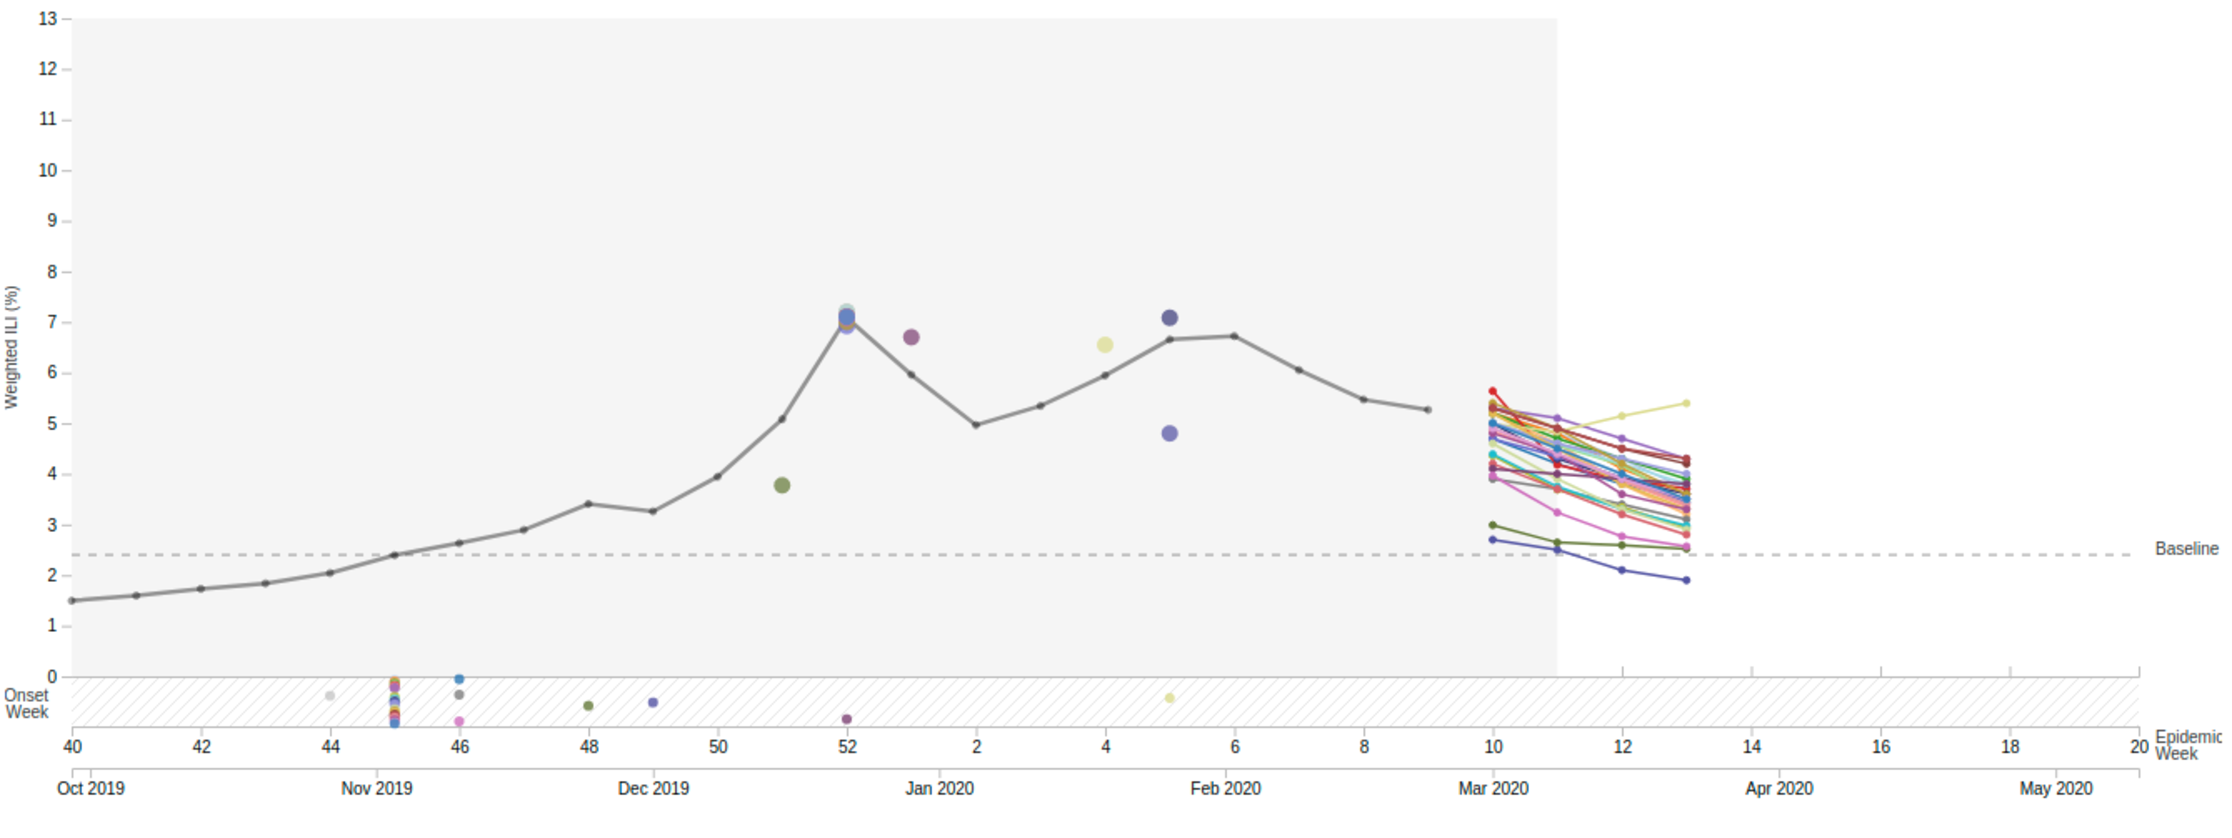
\includegraphics[scale=.3]{figures/flu_forecasts.pdf}
 \end{center}

\end{figure}

\end{frame}
%%%%%%%%%%%%%%%%%%%%%%%%%%%%%%%%%%%
\begin{frame}{Fixing notation}
%  \href{}{};

Let $\mathcal{P}$ be a convex class of probability measures on $(\Omega, \mathcal{A})$.
We call $P \in \mathcal{P}$ a probabilistic forecast. 
\begin{definition}[Scoring rule]
 We say $S(P, \cdot) : \Omega \to [-\infty, \infty]$ is a~\textbf{scoring rule} if it is measurable and $S(P, \cdot)$ is $P$-quasi-integrable for all $P \in \mathcal{P}$.
\end{definition}
The expected score under $Q \in \mathcal{P}$ if the forecast is $P$ is
\begin{equation}
 \nonumber
 S(P, Q) := \int_{\Omega} S(P, \omega)dQ(\omega). 
\end{equation}

\begin{definition}[Strictly proper scoring rule]
We say $S$ is~\textbf{proper} if $S(Q, Q) \geq S(P, Q)$ for all $P, Q \in \mathcal{P}$.
In addition, we say $S$ is~\textbf{strictly proper} if equality is achieved only for $P = Q$.
\end{definition}
\end{frame}
%%%%%%%%%%%%%%%%%%%%%%%%%%%%%%%%%%%
\begin{frame}
 \begin{definition}[Strong equivalence]
 If $S$ is a (strictly) proper scoring rule and $c\geq1$ is a constant and $h$ is a $\mathcal{P}$-integrable function, then~\href{https://sites.stat.washington.edu/raftery/Research/PDF/Gneiting2007jasa.pdf}{Gneiting \& Raftery, (2007)}, Eq.2: 
 \begin{equation}
  \label{eq:strongly_equiv}
  S^\ast(P, \omega) = c S(P, \omega) + h(\omega)
 \end{equation}
is also a (strictly) proper scoring rule and we say $S^\ast$ and $S$ are~\textbf{strongly equivalent} if $c = 1$.
\end{definition}
\textbf{Connection with convex functions:}
% First, two definitions:
% \begin{definition}[Sub-tangent]
%  A function $G^\ast(P, \cdot) : \Omega \to \bar{\mathbb{R}}$ is a~\textit{subtangent} of $G$ at $P \in \mathcal{P}$ if it is $P$-integrable, quasi-integrable with respect to all $Q \in \mathcal{P}$
% \end{definition}
% 
% \begin{definition}[Regular scoring rules]
%  We say a scoring rule  $S: \mathcal{P}\times \Omega \to \bar{\mathbb{R}}$ is~\textit{regular} relative to the class $\mathcal{P}$ if $S(P, Q)$ is real-valued for all $P, Q \in \mathcal{P}$, execpt perhaps for $S(P, Q) = -\infty$ if $P\neq Q$.
% \end{definition}
\begin{theorem}[Convex functions and proper scoring rules]
 A regular scoring rule $S: \mathcal{P}\times \Omega \to \bar{\mathbb{R}}$ is proper relative to the class $\mathcal{P}$ if and only if there exists convex $G : \mathcal{P} \to \mathbb{R}$ such that
 \begin{equation*}
  S(P, \omega) = G(P) - \int G^\ast (P, \omega)dP(\omega) + G^\ast(P, \omega),
 \end{equation*}
where $G^\ast(P, \omega)$ is a subtangent of $G$ at $P$.
\end{theorem}
\end{frame}
%%%%%%%%%%%%%%%%%%%%%%%%%%%%%%%%%%%
\begin{frame}{Information measures and (Bregman) divergences}
 The function 
 \begin{equation}
  G(P) = \sup_{Q \in \mathcal{P}} S(Q, P), P \in \mathcal{P}
 \end{equation}
 is the~\textbf{information measure} (or generalised entropy function) associated with $S$.
 Subject to regularity conditions on $S$, we can define
 \begin{equation}
 d(P, Q) = S(Q, Q) - S(P, Q),\: P,Q \in \mathcal{P},
\end{equation}
as the~\textbf{divergence function} associated with $S$ (and $G$).
Under regularity conditions on $\Omega$, $d(\cdot, \cdot)$ is called a~\textit{Bregman} divergence.

\textbf{Note:} if $S$ is strictly proper, $d(P, Q) \geq 0$ with equality iff $P = Q$.
\end{frame}
%%%%%%%%%%%%%%%%%%%%%%%%%%%%%%%%%%%
\section{Examples}
\begin{frame}{A first ``example''}
\textbf{Statistical decision problems}.
If we let $U(\omega, a)$ be the utility for outcome $\omega$ under action $a$ and $\mathcal{P}$ be a convex family of probability measures, then
\[ S(P, \omega) = U(\omega, a_P),\]
where $a_P$ is the Bayes act for $P \in \mathcal{P}$, is a proper scoring rule.
\end{frame}
%%%%%%%%%%%%%%%%%%%%%%%%%%%%%%%%%%%
\begin{frame}{Skill scores}
If we want to rank $n$ forecasts,~\textit{as long as they refer to the~\underline{same} set of forecast situations}, we can compute
\[ \mathcal{S}_n := \frac{1}{n}\sum_{i=1}^n S(P_i, x_i).\]

Since forecasts are likely to vary -- in quality -- spatially and temporally, we can compute the~\textbf{skill score}
\begin{equation}
 \mathcal{S}_n^{\text{skill}} := \frac{\mathcal{S}_n^{\text{fcst}} - \mathcal{S}_n^{\text{ref}}}{\mathcal{S}_n^{\text{opt}} - \mathcal{S}_n^{\text{ref}}},
\end{equation}
where 
\begin{itemize}
 \item $\mathcal{S}_n^{\text{fcst}}$ is the forecaster's score;
 \item $\mathcal{S}_n^{\text{opt}}$ is a hypothetical optimal forecast;
 \item $\mathcal{S}_n^{\text{ref}}$ is the score for a reference (model or) strategy.
\end{itemize}
\end{frame}
%%%%%%%%%%%%%%%%%%%%%%%%%%%%%%%%%%%
\begin{frame}{A slightly more enlightening example}
Suppose $\Omega = \{1, 2, \ldots, m\}$ consisting of mutually exclusive events and that $\mathcal{P}$ is the set of open $m-$dimensional unit simplices. 
If a forecaster quotes a vector $\boldsymbol{p} \in \mathcal{P}$ and event $i$ materialises, then their reward is $S(\boldsymbol{p}, i)$.

\begin{remark}[Convexity]
A (regular) scoring rule is proper if and only if $G(\boldsymbol{p}) = S(\boldsymbol{p}, \boldsymbol{p})$ is convex.
\end{remark}

\textbf{Example:} Brier score.
If $G(\boldsymbol{p}) = \sum_{j=1}^m p_j^2 - 1$, then we have the~\textit{Brier score}:
\begin{equation}
 S(\boldsymbol{p}, i) = -\sum_{j=1}^m \left(\mathbb{I}_j(i) - p_j\right)^2 - \sum_{j=1}^m p_j^2 - 1
\end{equation}

\end{frame}
%%%%%%%%%%%%%%%%%%%%%%%%%%%%%%%%%%%
\begin{frame}{More categorical examples}
\begin{itemize}
 \item \textbf{Spherical score}. 
 
 For $\alpha >1$ we can define
 \begin{equation}
  S(\boldsymbol{p}, i) = \frac{p_i^{\alpha -1}}{\left(\sum_{j=1}^m p_j^\alpha\right)^{\frac{\alpha-1}{\alpha}}}
 \end{equation}
\item \textbf{Logarithmic score}.

When $G(\boldsymbol{p}) = $ is the Shannon entropy, we have $S(\boldsymbol{p}, i) = \log p_i$ and 
\begin{equation}
 d(\boldsymbol{p}, \boldsymbol{q}) = \sum_{j=1}^m \log\left(\frac{q_j}{p_j}\right),
\end{equation}
as the Kullback-Leibler divergence.
\end{itemize}
\end{frame}
%%%%%%%%%%%%%%%%%%%%%%%%%%%%%%%%%%%
\begin{frame}{A (helpful?) visualisation}
\begin{figure}
 \begin{center}
  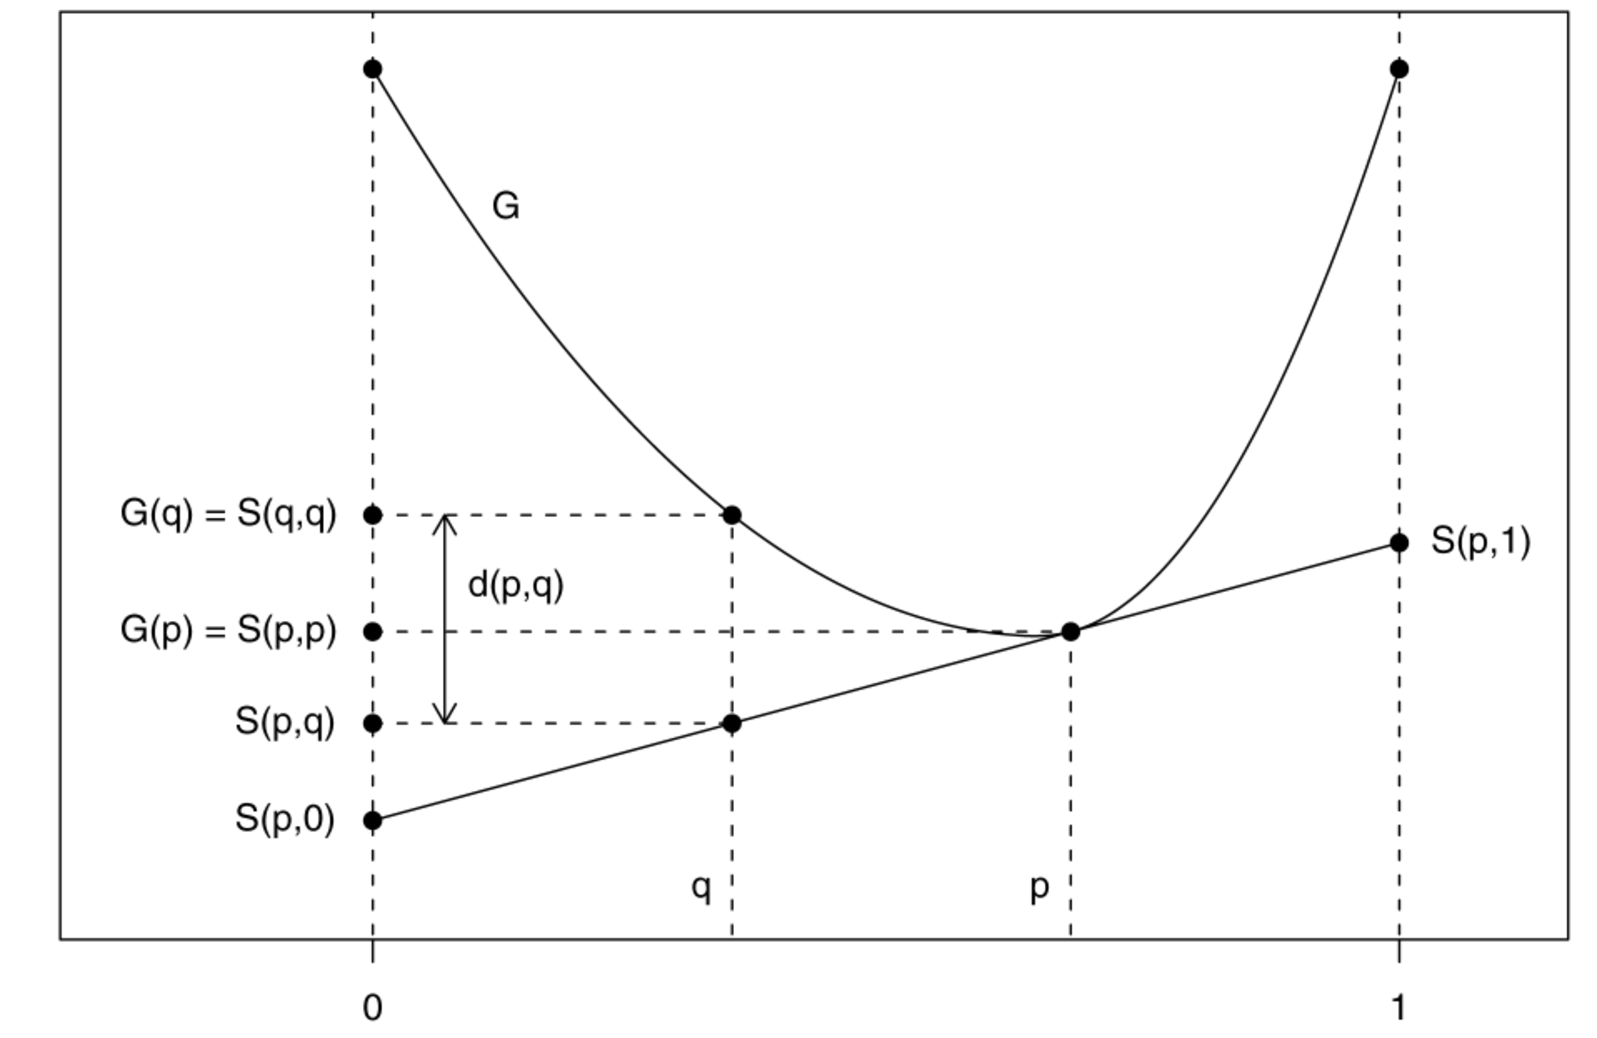
\includegraphics[scale=0.42]{figures/generalised_entropy.pdf}
 \end{center}
\end{figure}
\end{frame}
%%%%%%%%%%%%%%%%%%%%%%%%%%%%%%%%%%%
\begin{frame}{Scoring rules for density forecasts}

Let $\mu$ be a $\sigma$-finite measure on $(\Omega, \mathcal{A})$. 
For $\alpha > 1$ define $\mathcal{L}_\alpha$ be the space of probability measures on $(\Omega, \mathcal{A})$ such that $\nu \ll \mu$ and $p(\omega) = \frac{d \nu}{d \mu}(\omega)$ and 
\begin{equation}
\nonumber
 ||p||_\alpha = \left( \int_{\Omega} p(\omega)^\alpha d\mu(\omega) \right)^\alpha < \infty.
\end{equation}

We establish a correspondence between the forecast $P$ and its $\mu$-density, $p$.
\textbf{Examples:}
\begin{itemize}
 \item \textbf{Quadratic:}
 
 \begin{equation}
  \operatorname{QS}(p, \omega) = 2p(\omega) - ||p||_2^2,
 \end{equation}
is strictly proper relative to $\mathcal{L}_2$ class of probability measures. 

\item \textbf{Pseudo-spherical:}
 \begin{equation}
  \operatorname{PseudoS}(p, \omega) = \frac{p(\omega)^{\alpha-1}}{||p||_{\alpha}^{\alpha-1}},
 \end{equation}
\item \textbf{Logarithmic score:}

 \begin{equation}
  \operatorname{LogS}(p, \omega) = \log p(\omega),
 \end{equation}
 is what happens to the pseudo-spherical score when $\alpha \to 1$.
\end{itemize}
\end{frame}
%%%%%%%%%%%%%%%%%%%%%%%%%%%%%%%%%%%
\begin{frame}{Illustrations: $G(p)$}
\begin{figure}
 \begin{center}
  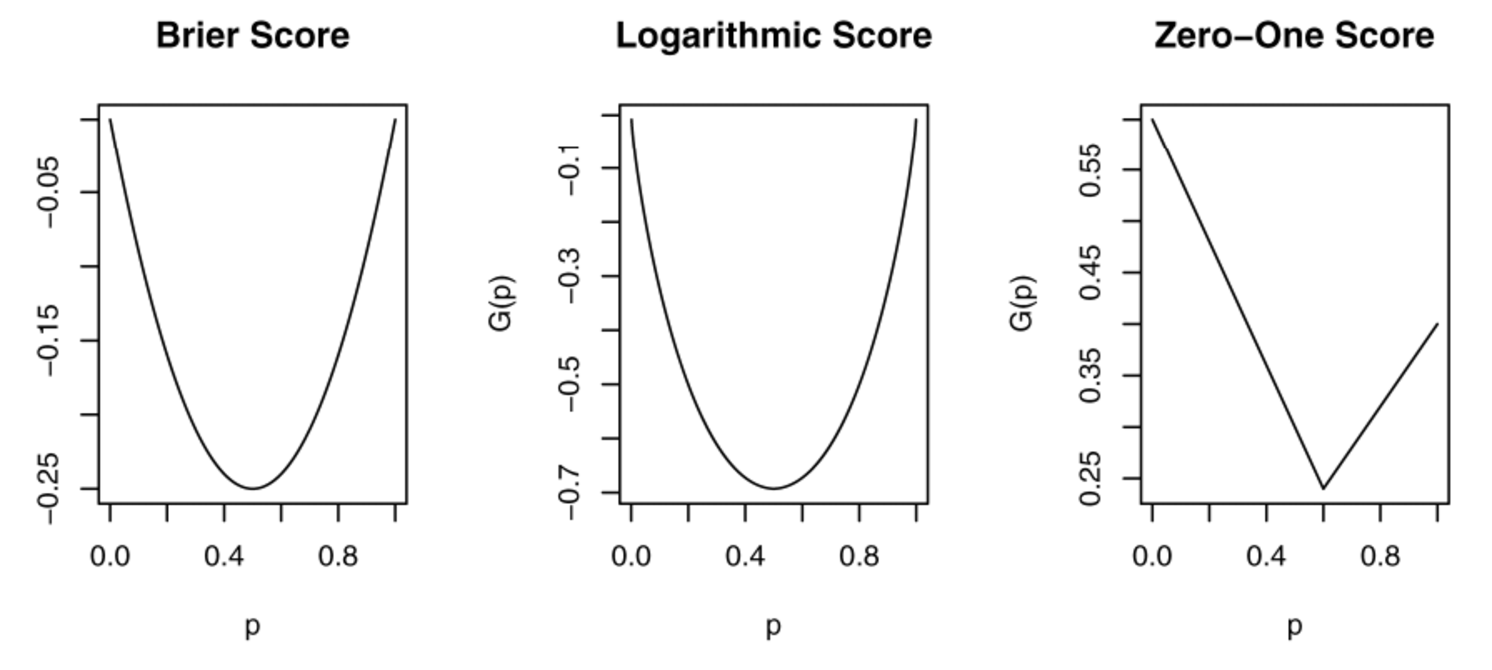
\includegraphics[scale=0.45]{figures/G_of_p.pdf}
 \end{center}
\end{figure}
\end{frame}
%%%%%%%%%%%%%%%%%%%%%%%%%%%%%%%%%%%
\begin{frame}{Illustrations: $S(p, 1)$ and $S(p, 0)$}
\begin{figure}
 \begin{center}
  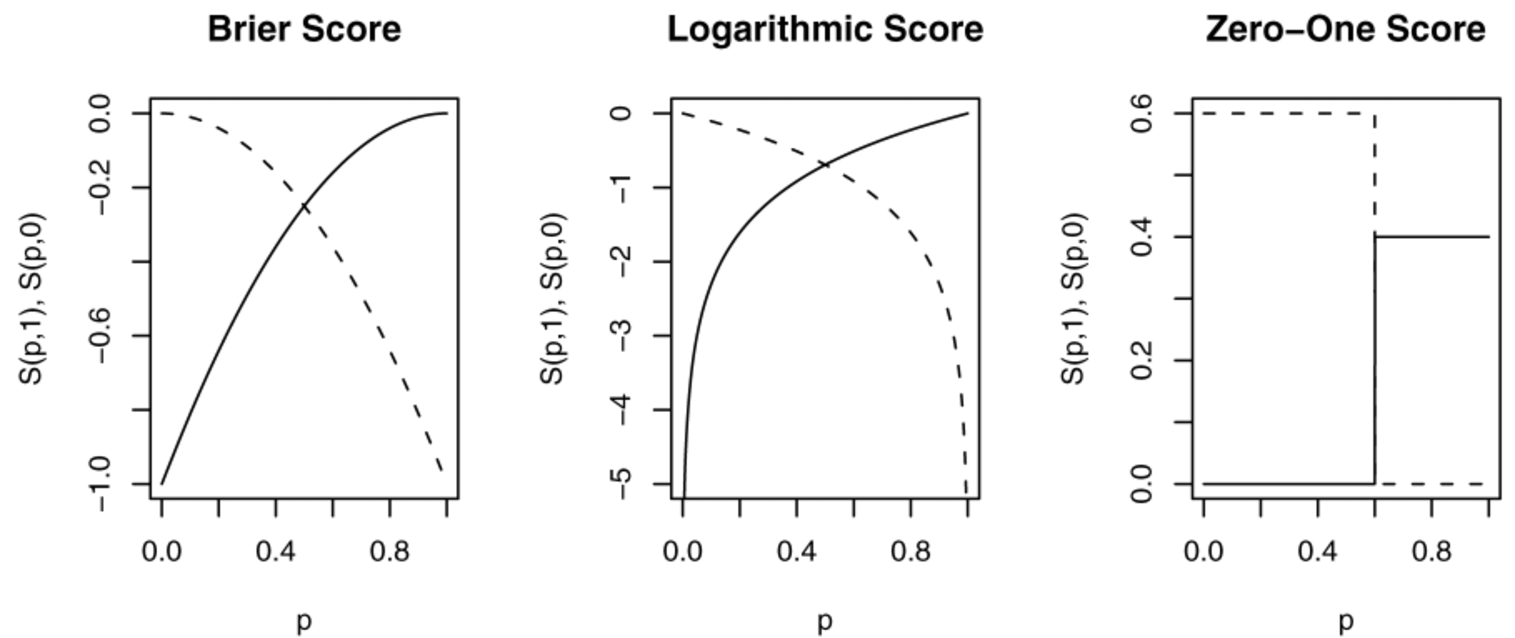
\includegraphics[scale=0.45]{figures/S_of_p.pdf}
 \end{center}
\end{figure}
\end{frame}
%%%%%%%%%%%%%%%%%%%%%%%%%%%%%%%%%%%
\begin{frame}{Continuous ranked probability score}
The continuous ranked probability score (CRPS):
\begin{equation}
 \operatorname{CRPS}(F, x) = -\int_{-\infty}^{\infty} \left( F(y) - \mathbb{I}\{y \geq x\}\right)^2\,dy,
\end{equation}
can be seen as the integral of the Brier scores for the associated binarisation of the forecasts based on $x$ as cutoff.

\textbf{Example:}
\begin{equation*}
 \operatorname{CRPS}\left(\text{Normal}(\mu, \sigma^2), x\right) = \sigma \left[ \frac{1}{\sqrt{\pi}}-2\varphi\left(\frac{x-\mu}{\sigma}\right) - \frac{x-\mu}{\sigma}\left(2\Phi\left(\frac{x-\mu}{\sigma}\right)-1\right) \right],
\end{equation*}
where $\varphi$ and $\Phi$ are the probability density function and cumulative distribution function of a standard normal, respectively.
\end{frame}
%%%%%%%%%%%%%%%%%%%%%%%%%%%%%%%%%%%
\begin{frame}{Loads more!}
The article lists a bunch more scoring rules:
\begin{itemize}
 \item Energy score (Section 4.3), a generalisation of CRPS;
 \item Scoring rules that depend on the first two moments only (Section 4.4);
 \item Kernel scores (Section 5) -- negative-definite functions and (Hoeffding) expectations inequalities;
 \item Random-fold cross-validation (Section 7.2).
\end{itemize}
\end{frame}
%%%%%%%%%%%%%%%%%%%%%%%%%%%%%%%%%%%
\begin{frame}{Quantiles and Bayes factors}
A few more connections.

\begin{itemize}
 \item \textbf{Quantiles:}

 If one quotes the quotes the quantiles $r_1, \ldots, r_k$, we have
\begin{equation*}
 S(r_1, \ldots, r_k; P) = \int S(r_1, \ldots, r_k; x)\,dP(x)
\end{equation*}
as a proper scoring rule under somewhat mild technical conditions (see Theorem 6 in~\href{https://sites.stat.washington.edu/raftery/Research/PDF/Gneiting2007jasa.pdf}{Gneiting \& Raftery, (2007)}). 
  \item \textbf{Bayes factors:}
 
 We have
 $$B_{12} = \frac{P(\boldsymbol{X} \mid H_1)}{P(\boldsymbol{X} \mid H_2)},$$
 and thus 
 $$\log B_{12} = \operatorname{LogS}(H_1, \boldsymbol{X}) - \operatorname{LogS}(H_2, \boldsymbol{X}), $$
 is a proper scoring rule.
\end{itemize}
\end{frame}
%%%%%%%%%%%%%%%%%%%%%%%%%%%%%%%%%%%
\begin{frame}{Case study I: interval forecasts for heterokedastic processes}
 The (Markovian) model is
 \[X_{t+1} = \frac{1}{2}X_t + \frac{1}{2}X_t \epsilon_t + \epsilon_t,\: \epsilon_t \sim \operatorname{Normal}(0, 1).  \]
 
 Interval predictions for $X_{t+1}$ will be
 \begin{equation}
  I := \left[\frac{1}{2}X_t - c \left|1 + \frac{1}{2}X_t\right|,  \frac{1}{2}X_t + c \left|1 + \frac{1}{2}X_t\right| \right],
 \end{equation}
with $c = \Phi^{-1}( \frac{1 + \alpha}{2})$ and $\alpha = 0.95$.

Alternative forecast is 
\begin{equation}
 J := \left[F^{-1}\left(\frac{1 - \alpha}{2}\right), F^{-1}\left(\frac{1 + \alpha}{2}\right) \right],
\end{equation}
where $F$ is the unconditional stationary distribution of $X_t$.
Finally, consider also 
\begin{equation}
  K := \left[\frac{1}{2}X_t - \gamma\left(\left|1 + \frac{1}{2}X_t\right|\right),  \frac{1}{2}X_t + \gamma\left(\left|1 + \frac{1}{2}X_t\right|\right) \right]
\end{equation}
where $\gamma(a) = a\sqrt{2\left(\log 7.36 - \log a\right)} \mathbb{I}(a < 7.26)$, which minimises interval width subject to nominal coverage.
\end{frame}
%%%%%%%%%%%%%%%%%%%%%%%%%%%%%%%%%%%
\begin{frame}{Results I}
 \begin{figure}
 \begin{center}
  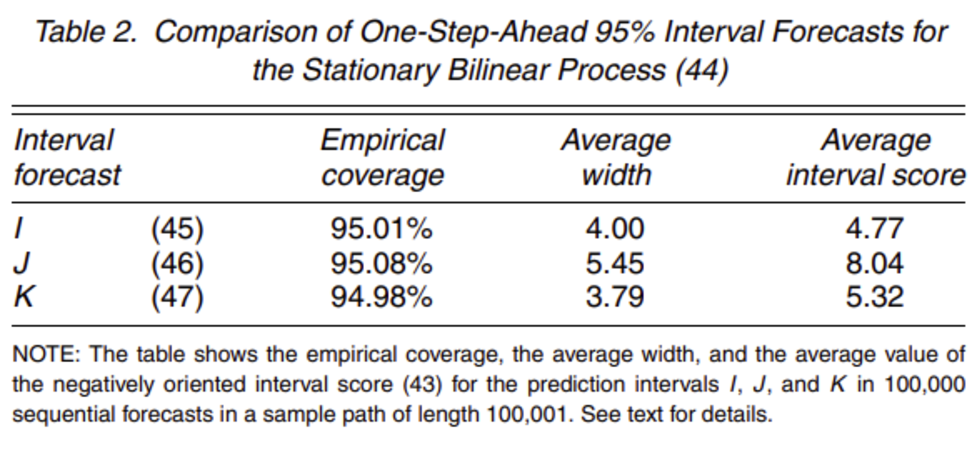
\includegraphics[scale=0.5]{figures/heterokedastic.pdf}
 \end{center}
\end{figure}
\end{frame}
%%%%%%%%%%%%%%%%%%%%%%%%%%%%%%%%%%%
\begin{frame}{Case study II: forecasting sea-level pressure}
 Key idea:~\textbf{model ensembles}.
 
 Five models give 48-hour look ahead predictions for sea-level pressure in (some places of) the Pacific Ocean. 
 
 \textbf{Problem:} underdispersed predictions by the ensemble.
 
 \textbf{Solution:} Come up with an inflation factor ($R$).
 
 \begin{figure}
 \begin{center}
  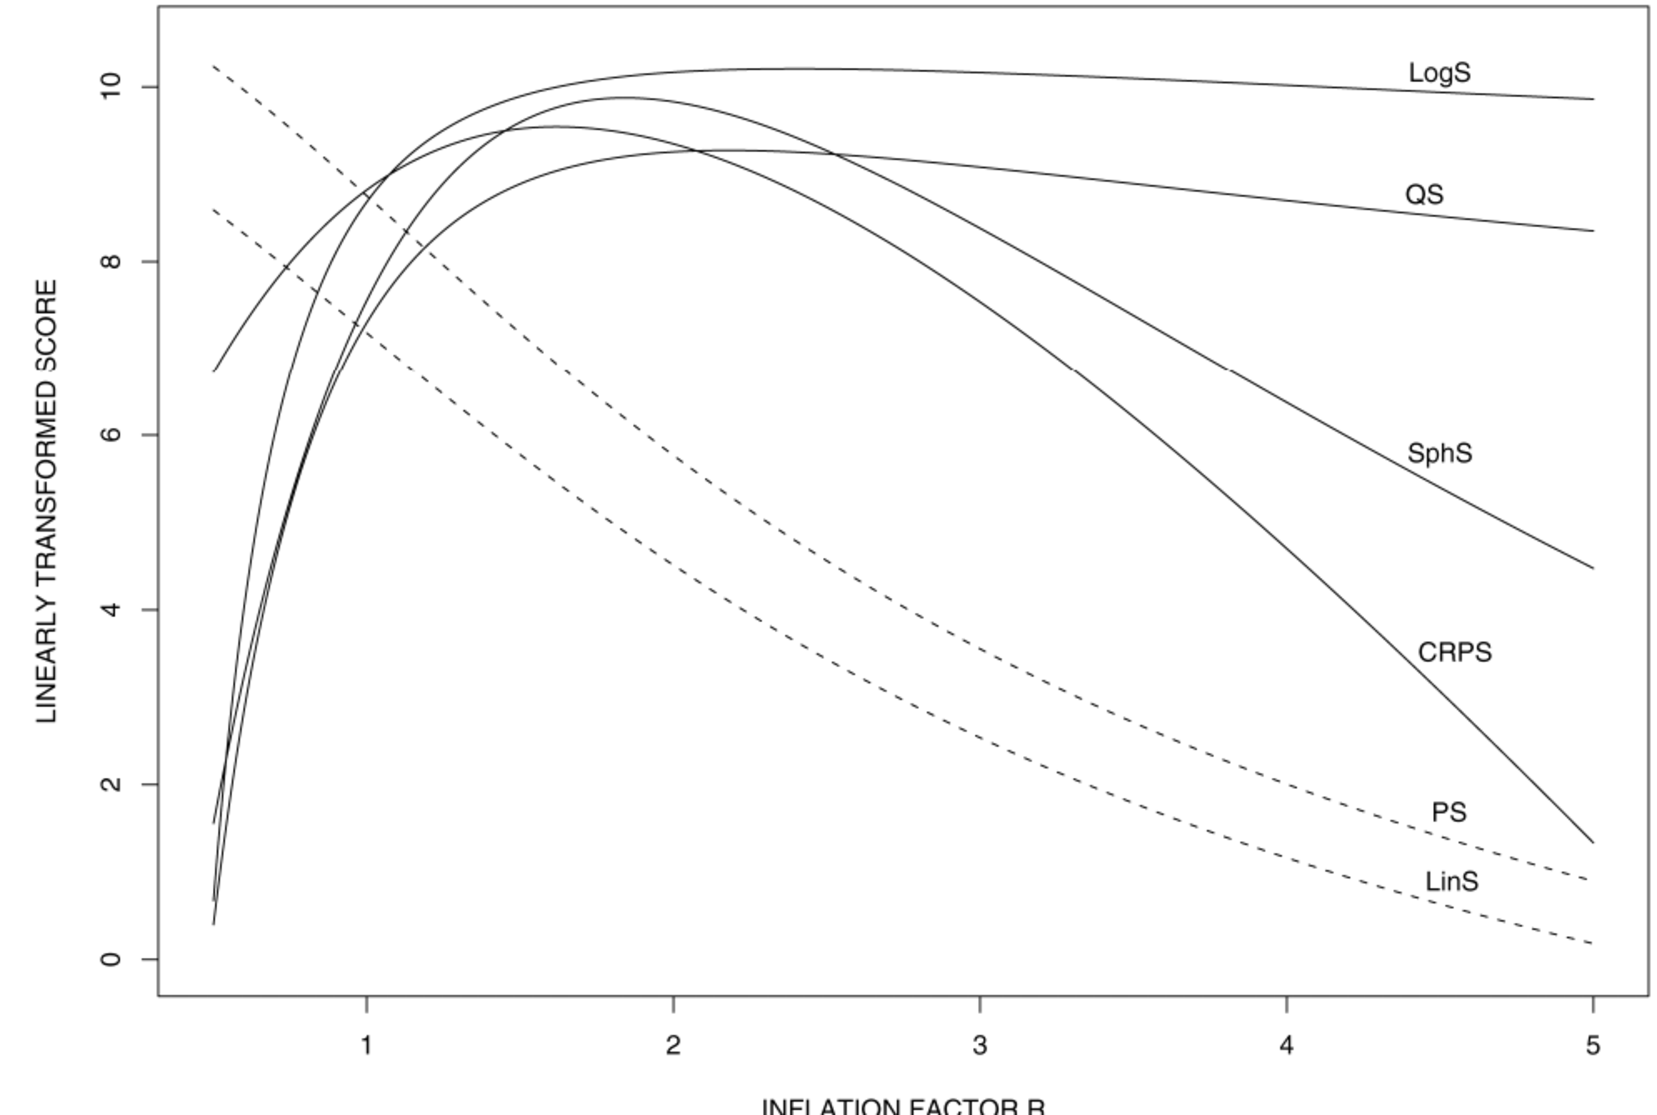
\includegraphics[scale=0.3]{figures/sealevelpressure.pdf}
 \end{center}
\end{figure}
 
\end{frame}
%%%%%%%%%%%%%%%%%%%%%%%%%%%%%%%%%%%
\begin{frame}{Results IIb}
 For upper ($u_i$) and lower ($l_i$) predictions, we can evaluate interval forecasts for the sea-level pressure problem using, for $r>0$,
 \[ s_{\alpha}(r) = \frac{1}{16 ,015}\sum_{i=1}^{16 ,015} S_{\alpha}^{\text{int}}(l_i, u_i; x), \]
 as a scoring rule, which takes both calibration and sharpness into account.

 \begin{figure}
 \begin{center}
  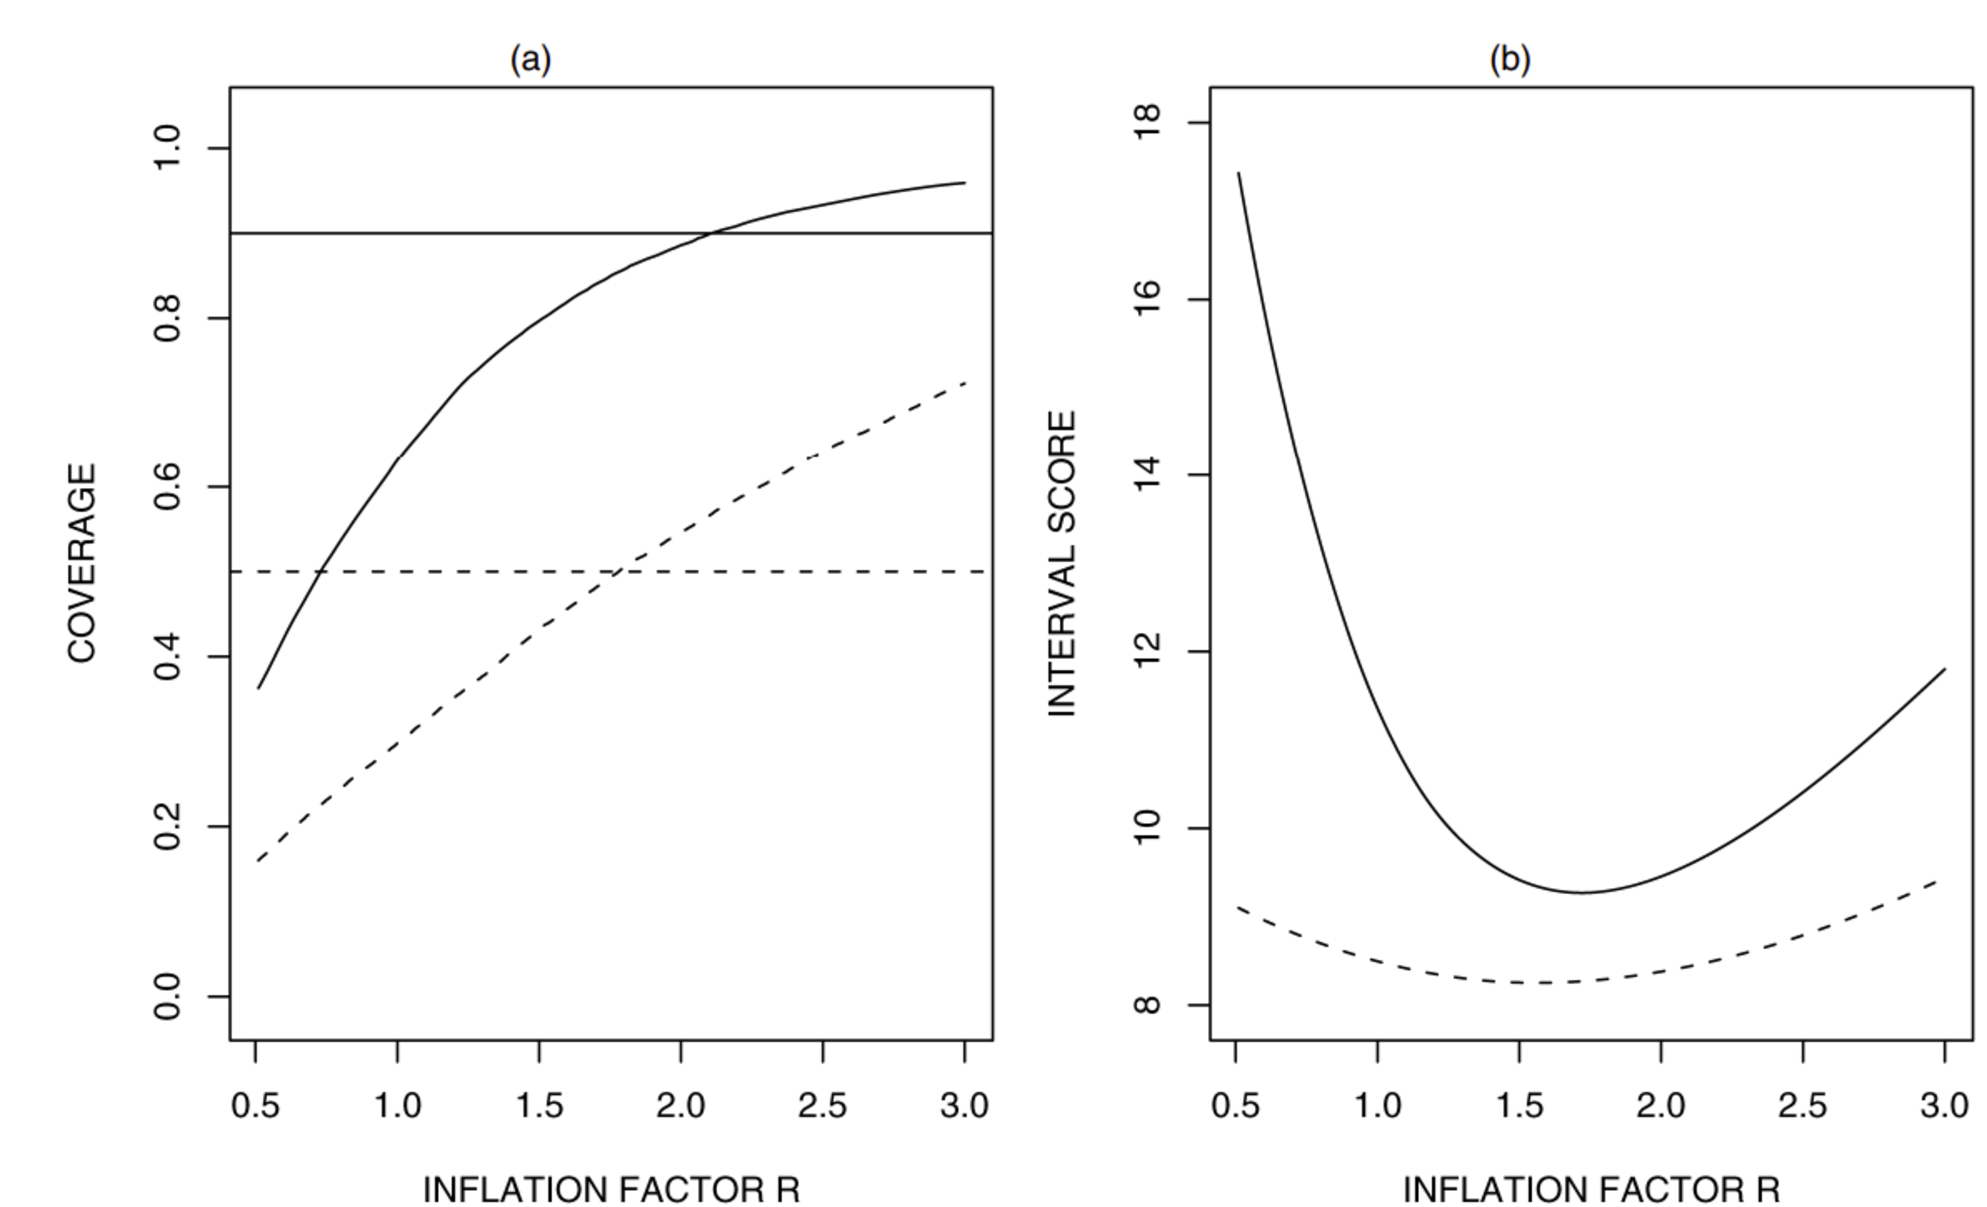
\includegraphics[scale=0.25]{figures/sealevelpressure2.pdf}
 \end{center}
\end{figure}
\end{frame}


%%%%%%%%%%%%%%%%%%%%%%%%%%%%%%%%%%%
\begin{frame}{Applications in Epidemiology}
\begin{itemize}
 \item The obvious: assess COVID-19 forecasts;
 \item The not-so-obvious: InfoDengue and InfoGripe (``gripe'' is Portuguese for the flu);
\end{itemize} 
 \begin{figure}
 \begin{center}
  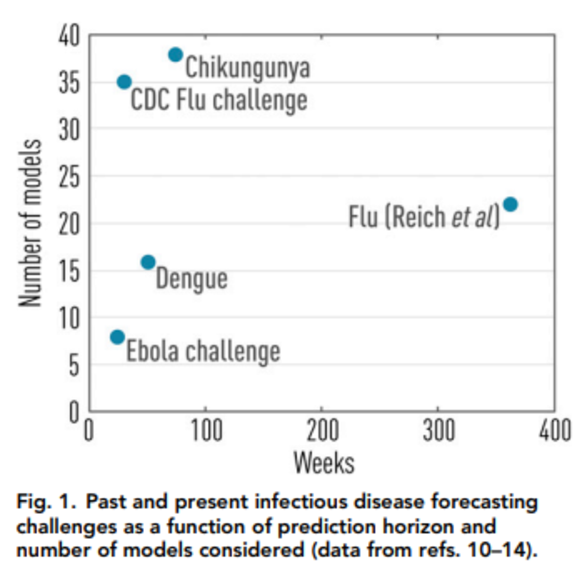
\includegraphics[scale=0.55]{figures/diseaseprediction.pdf}
 \end{center}
\end{figure}
Figure 1 of~\href{https://www.pnas.org/content/pnas/116/8/2802.full.pdf}{Viboud \& Vespigiani (2019).}

\end{frame}
%%%%%%%%%%%%%%%%%%%%%%%%%%%%%%%%%%%
\begin{frame}{Conclusions}
\begin{itemize}
 \item Proper scoring rules (PSRs) are cool! 
  They permeate many seemingly unrelated things;
 \item A proper scoring rule encourages honest and well-calibrated forecasts;
 \item It is possible to define PSRs for interval, point and distributional forecasts;
 \item For more, see the work by Alexander P. Dawid, starting with~\href{http://qwone.com/~jason/trg/papers/dawid-prequential-84.pdf}{Dawid (1984)}.
\end{itemize}

\end{frame}
%%%%%%%%%%%%%%%%%%%%%%%%%%%%%%%%%%%

\end{document}
